\documentclass[a4paper]{article}
\usepackage[spanish]{babel}
\usepackage[utf8]{inputenc}
\usepackage{charter}   % tipografia
\usepackage{graphicx}
%\usepackage{makeidx}
\usepackage{paralist} %itemize inline
\usepackage{algorithmicx}
\usepackage{algpseudocode}



%\usepackage{float}
%\usepackage{amsmath, amsthm, amssymb}
%\usepackage{amsfonts}
%\usepackage{sectsty}
%\usepackage{charter}
%\usepackage{wrapfig}
%\usepackage{listings}
%\lstset{language=C}


\usepackage{color} % para snipets de codigo coloreados
\usepackage{fancybox}  % para el sbox de los snipets de codigo

\definecolor{litegrey}{gray}{0.94}

% \newenvironment{sidebar}{%
% 	\begin{Sbox}\begin{minipage}{.85\textwidth}}%
% 	{\end{minipage}\end{Sbox}%
% 		\begin{center}\setlength{\fboxsep}{6pt}%
% 		\shadowbox{\TheSbox}\end{center}}
% \newenvironment{warning}{%
% 	\begin{Sbox}\begin{minipage}{.85\textwidth}\sffamily\lite\small\RaggedRight}%
% 	{\end{minipage}\end{Sbox}%
% 		\begin{center}\setlength{\fboxsep}{6pt}%
% 		\colorbox{litegrey}{\TheSbox}\end{center}}

\newenvironment{codesnippet}{%
	\begin{Sbox}\begin{minipage}{\textwidth}\sffamily\small}%
	{\end{minipage}\end{Sbox}%
		\begin{center}%
		\colorbox{litegrey}{\TheSbox}\end{center}}



\usepackage{fancyhdr}
\pagestyle{fancy}

%\renewcommand{\chaptermark}[1]{\markboth{#1}{}}
\renewcommand{\sectionmark}[1]{\markright{\thesection\ - #1}}

\fancyhf{}

\fancyhead[LO]{Sección \rightmark} % \thesection\ 
\fancyfoot[LO]{\small{Ángel Fernando More, Claudio Gomez, Fernando Otero}}
\fancyfoot[RO]{\thepage}
\renewcommand{\headrulewidth}{0.5pt}
\renewcommand{\footrulewidth}{0.5pt}
\setlength{\hoffset}{-0.8in}
\setlength{\textwidth}{16cm}
%\setlength{\hoffset}{-1.1cm}
%\setlength{\textwidth}{16cm}
\setlength{\headsep}{0.5cm}
\setlength{\textheight}{25cm}
\setlength{\voffset}{-0.7in}
\setlength{\headwidth}{\textwidth}
\setlength{\headheight}{13.1pt}

\renewcommand{\baselinestretch}{1.1}  % line spacing


% \setcounter{secnumdepth}{2}
\usepackage{underscore}
\usepackage{caratula}
\usepackage{url}


% ******************************************************** %
%              TEMPLATE DE INFORME ORGA2 v0.1              %
% ******************************************************** %
% ******************************************************** %
%                                                          %
% ALGUNOS PAQUETES REQUERIDOS (EN UBUNTU):                 %
% ========================================
%                                                          %
% texlive-latex-base                                       %
% texlive-latex-recommended                                %
% texlive-fonts-recommended                                %
% texlive-latex-extra?                                     %
% texlive-lang-spanish (en ubuntu 13.10)                   %
% ******************************************************** %



\begin{document}


\thispagestyle{empty}
\materia{Organizaci\'on del computador II}
\submateria{Segundo Cuatrimestre de 2014}
\titulo{Trabajo Pr\'actico III}
\integrante{Otero, Fernando Gabriel}{424/11}{fergabot@gmail.com}
\integrante{More \'Angel}{931/12}{angel\_21\_fer@hotmail.com}
\integrante{Gomez Arco Claudio}{312/13}{claudio4158@hotmail.com}

\maketitle
\newpage
\thispagestyle{empty}
\vspace{3cm}
\tableofcontents
\newpage


\newpage
\section{Ejercicio 1}
\subsection*{A)}
Utilizando el struct str\_gdt\_entry dada en $gdt.h$  completamos los primeros 8 (contando desde 0) descriptores con todos los campos en 0 ya que estos son descriptores nulos.\newline
En la posici\'on 9 est\'a el descriptor de c\'odigo de nivel 0. Este tiene que direccionar los primeros 624MB, pero como usamos granularidad tenemos que pasar la unidad de B a 4KB. 
Entonces la base es el resultado de esto (0x26EFF) y la acomodamos en las partes donde corresponde (porque est\'a "partida").
La base es 0. El tipo es A (ejecuci\'on y lectura). S (Descriptor type) es 1 porque es de tipo c\'odigo. Dpl es 0 porque es c\'odigo de nivel 0. D/b es 1 porque es para 32 bits. Presente est\'a en 1 porque lo vamos a usar. \newline
En la posici\'on 10 está lo mismo que en la posici\'on 9, pero dpl cambia a 3 porque es c\'odigo de nivel 3. \newline
En la posici\'on 11 est\'a el descriptor de datos de nivel 0, es lo mismo que en la posici\'on 9 pero cambiando tipo por 2 ya que es de lectura/escritura.\newline
En la posici\'on 12 está lo mismo que en la 11 pero cambia el dpl a 3 ya que el descriptor de datos es de nivel 3.
En la posici\'on 13 est\'a el descriptor de video, lo mismo que  en la posici\'on 12, cambiando la base por 0xB8000 y el dpl es 0. \newline

Luego para entender mejor que descriptor es cada posici\'on realizamos defines, en el archivo $defines.h$, para cada uno de ellos, as\'i tambi\'en sus offsets (posici\'on * 8).

\subsection*{B)}
En $kernel.asm$, habilitamos el pin A20 con call habilitar\_A20. Cargamos la gdt con LGDT y GDT\_DESC(función en $gdt.c$) ,luego seteamos el bit PE de CR0, e hicimos un JUMP 
para pasar a modo protegido en el segmento de c\'odigo nivel 0 (el jmp es necesario para cambiar el valor del registro $cs$).\newline
Luego, inicializamos los selectores de segmentos, data (ds) con el offset de la posici\'on 10 (datos de nivel 0), así también para todos los segmentos restantes menos para $fs$ que tiene el offset de la posici\'on 12(desciptor de video). 
Por \'ultimo pusimos en $esp$, y en $ebp$ 0x27000 (ya que la pila debe comenzar en esta direcci\'on).

\subsection*{C)}
Para describir el \'area de la pantalla en memoria, para ser utilizado por el Kernel, se declaro la entrada de la posici\'on 12 en la GDT, el mismo corresponde al segmento de 
video (Explicado en A) y el segmento correspondiente para video sera el fs, inicializado con el offset de dicha entrada.

\subsection*{D)}
Se procedio a limpiar la pantalla con el coloreo b\'asico, que es pintar todo el mapa de verde y las barras laterales de rojo y azul. Usando el segmento definido 
anteriormente. El pseudoc\'odigo para realizar esto es el siguiente: 
\begin{codesnippet}
\begin{verbatim}
    ; la pantalla esta representada por una mariz de tamaño 50x80 
    ; donde cada elemento ocupa 2 bytes
        xor ecx, ecx
        xor edx, edx 
	inc edx
	xor esi, esi
	add esi, 159
.ciclo: ;pinto de verde
	cmp ecx, 8000		;tamano de la pantalla
	je .ciclo2
	mov byte [fs:ecx], 0x22	;verde en el fondo
	inc ecx		;avanzo en la matriz
	jmp .ciclo	
.ciclo2: ; pinto barras
	cmp edx, 8000
	jae .mapa_ok
	mov byte [fs:edx], 0x44	;rojo
	mov byte [fs:esi], 0x11	;azul
	add edx, 160 
	add esi, 160
	jmp .ciclo2
.mapa_ok:

\end{verbatim}
\end{codesnippet}
\newpage
\section{Ejercicio 2}
\subsection*{A)}
Utilizamos la macro dada en isr.asm, que dado un entero crea un c\'odigo \_isr(). Esta funci\'on llamar\'a a la funcion en C $mostrarError$, luego desalojar\'a la  tarea actual y 
por ultimo pasar\'a a la tarea idle, si esta no es la tarea actual.

\begin{codesnippet}
\begin{verbatim}
%macro ISR 1
global _isr%1

_isr%1:
    mov EAX, %1
    PUSH EAX
    CALL mostrarError
    pop eax
.fin:
    call desalojar_tarea
    
    mov dword [estaIdle], 0x1
    mov dword [selector], 0x70
	jmp far [offset]
    iret
%endmacro
\end{verbatim}
\end{codesnippet}

MostrarError es un switch case, que dado un entero entre 0 y 20 mapea un error a un mensaje(descripci\'on) y lo imprime por pantalla con la funci\'on print dada en screen.c, 
y por ultimo llama a la funcion $mDebugger()$.
Luego utilizamos la macro ISR para $i$, $i= 0..20$
En isr.h llamamos a \_isr($i$), para $i= 0..20$, ya que esto ser\'a utilizado por idt.c, para obtener el offset de la rutina encargada de atender la interrupci\'on. \newline
Por \'ultimo en idt.c inicializamos el arreglo de interrupciones con la funci\'on $idt\_inicializar$. Para esto, a su vez inicializamos a cada interrupci\'on dentro del mismo 
por medio de una macro, \#$define$ $IDT\_ENTRY(numero)$. La misma se encarga de completar todos los campos que poseen los descriptores de segmento de las interrupciones. 
Un offset que es la direcci\'on de la funci\'on \_isr correspondiente; segsel que se corresponde al segmento de c\'odigo nivel cero. Y los atributos 
P=1; dpl correspondiente a la tarea y d= 1 (para 32bits). 

\subsection*{B)}
En kernel.asm llamamos a idt\_inicializar(función en $idt.c$), que completa el vector de interupciones de las posiciones 0 a 19, 32, 33 y 102 con \#define IDT\_ENTRY(numero) de la 
forma descripta en el punto $A$.

 
 
  La entrada 102 es la interrupción $mover$, la cual es llamada por las tareas. Por eso pusismos los atributos correspondientes (0xEE00) para que sea de 
nivel 3\color{black} . Luego con LIDT cargamos el vector de interrupciones(idt_entry en $idt.h$) utilizando la estructura IDT_DESC definido en $idt.c$.

\newpage
\section{Ejercicio 3}
\subsection*{A)}
Para terminar de pintar la pantalla creamos una funci\'on en screen.c, iniciarPantalla. El pseudoc\'odigo de la misma es el siguiente:
\begin{codesnippet}
\begin{verbatim}
void iniciar_pantalla()
{	
	clockd[0] = '|';
	clockd[1] = '/';
	clockd[2] = '-';
	clockd[3] = '\\';
	Debugger = 0;
	
	unsigned int x,y;
	const char* texto = " ";
	//Los espacios en negro:
	for (x = 0; x < 80; x++)
	{
			print(texto, x, 0, 0x00);
			print(texto, x, 45, 0x00);
			print(texto, x, 46, 0x00);
			print(texto, x, 47, 0x00);
			print(texto, x, 48, 0x00);
			print(texto, x, 49, 0x00);	
	} 
	
	for (x = 35; x < 45; x++)
	{
		for (y = 45; y < 50; y++)
		{
			if (x < 40)
			{
				print(texto, x, y, 0x44);	//Franja roja (4 = rojo)
			}
			else
			{
				print(texto, x, y, 0x11);	//Franja azul (1 = azul)
			}
		}	
	}
\end{verbatim}
\end{codesnippet}
\begin{codesnippet}
\begin{verbatim}
	texto = "1 2 3 4 5 6 7 8";
	print(texto, 5, 46, 0x0f);
	print(texto, 60, 46, 0x0f);
	print("( )", 75, 49, 0x0f);
	texto = "# # # # # # # #";	//relojes
	print(texto, 5, 48, 0x0f);
	print(texto, 60, 48, 0x0f);

	print("G", 0, 1, 0x44);
	print("G", 79, 1, 0x11);
	
	puntaje_o_restantes(juego.puntaje_B , 41, 47, 0x1f);
	puntaje_o_restantes(juego._20A, 31, 47, 0x4f);
	puntaje_o_restantes(juego.puntaje_A , 36, 47, 0x4f);
	puntaje_o_restantes(juego._20B, 49, 47, 0x1f);
	
}
\end{verbatim}
\end{codesnippet}

\subsection*{B)}

El procesador posee una unidad de manejo de memoria, MMU, (Memory Management Unit) que es un dispositivo de Hardware responsable del manejo de los accesos a memorias, entre 
algunas de sus funciones. Este dispositivo se va a encargar  de la traducci\'on de las direcciones l\'ogicas (o virtuales) a direcciones f\'isicas (o reales) que enviara por el 
bus de address hacia la memoria externa. Para representar esto se cuenta  con un directorio de paginas, cada pagina tiene un tamaño de 4k y 1024 descriptores de 8 bytes. Cada uno 
representa en los bits 31 a 12  el valor correspondiente a la direcci\'on f\'isica de la Pagina (el Page Frame) que contiene la tabla de descriptores de pagina, cada una de estas 
con 1024 descriptores. Adem\'as  cada descriptor de 32 bits posee las siguientes caracter\'isticas:\newline

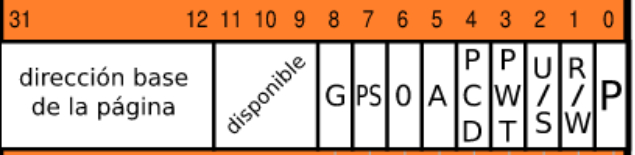
\includegraphics[width=\textwidth,height=1.0in,keepaspectratio
]{imagen.jpg}\newline

Para representar los descriptores y con esto el directorio de paginas se utilizo un str en lenguaje C, como el que se muestra a continuaci\'on y en el archivo mmu.c		\newline
\begin{codesnippet}
\begin{verbatim}
typedef struct str_mmu_entry{ 
	\textit{	unsigned char p:1;
		unsigned char rw:1; 
		unsigned char us:1; 
		unsigned char pwt:1;
		unsigned char pcd:1; 
		unsigned char a:1; 
		unsigned char ign:1;
		unsigned char ps:1; 
		unsigned char g:1;
		unsigned char disp:3; 
		unsigned int  base\_0\_20  :20; }
} \textit{__attribute__((__packed__, aligned (4))) mmu_entry};
\end{verbatim}
\end{codesnippet}
estructura que representa un descriptor de directorio de pagina y de la page table. Si bien entre si difieren algunos de sus par\'ametros, los que lo hacen no se utilizan.\newline \newline

\subsubsection*{mmu\_inicializar\_dir\_kernel()}
En la page table  cada descriptor, con el atributo P=1, contiene la direcci\'on de una pagina  correspondiente  a una Tabla de Paginas. Este es el ultimo nivel de traducci\'on. Cada pagina es de 4K, con 1024 descriptores de 4bytes cada uno. Y cada uno de estos posee en los  bits 31 a 12,  el Page Frame de la pagina de memoria, es decir los 20 bits mas significativos de la direcci\'on f\'isica de memoria en donde comienza la pagina.\newline
Como se desea crear un directorio de paginas que mapee usando identity mapping, las direcciones 0x00000000 a 0x3FFFFF, se necesita completar 1 pagina, de la page table  ya que cada descriptor se corresponde con un pagina en direcci\'on f\'isica de 4K y en total se estar\'ian completando  1024 descriptores, como cada uno se corresponde con 4k obtenemos 1024*4  = 0x400000 que es  lo que necesitamos direccionar.  Como fue necesaria una pagina,  se completó un  descriptor de la page directory  con los siguientes atributos (la inicializaci\'on de todos las paginas y descriptores mencionados se encuentran mmu.c). En primer lugar se declaro que la direcci\'on inicial del directorio de pagina es la 0x27000: \textit{ mmu\_entry *pd = ( mmu\_entry *) 0x27000; p = 1; rw = 1; us = 0; pwt = 0; pcd = 0; a = 0;  ign = 0; ps = 0; g = 0; disp = 0;} debido a que los 20 bits mas significativos constituyen la  direcci\'on del directorio de pagina, se shiftea 12 bits hacia la izquierda para quedarnos con los restantes $base\_0\_20$ = (0x28000 + i*0x1000) $>>$ 12;  \newline
Como cada pagina posee 1024 descriptores, el resto de los descriptores sin usar fueron inicializados con los mismo atributos excepto que P=0 , ya que no se necesitan.
Una vez realizado esto se inicializaron los ya mencionados descriptores de pagina.  Como ya se cuenta con un directorio de pagina inicializado en la direcci\'on 0x27000 y esta ocupa 0x1000, las tablas de pagina van a comenzar a partir de la direcci\'on 0x28000. Y los atributos tendr\'an el valor \textit{mmu\_entry *pt = (mmu\_entry *) 0x28000 ; p = 1; rw = 1; us = 0; pwt = 0; pcd = 0; a = 0; ign = 0; ps = 0; g = 0; disp = 0; base\_page\_0\_20 = i*0x1000}; Donde 0 $<=$ i $<=$ 1024, ya que de esta manera se direcciona a los primero 4Mb de memoria.\newline \newline

\subsection*{C)}
En $kernel.asm$ llamamos a mmu\_inicializar lo que hace es empezar un contador de páginas libres. Llamamos a mmu\_inicializar\_dir\_kernel que hace lo descripto arriba. \newline
Colocamos en CR3 0x27000 porque es donde empieza la page directory y seteamos el primer bit de CR0, todo esto para habilitar paginación. 


\subsection*{D)}
Creamos un texto con el nombre del grupo de la misma forma que estaba hecho para \newline$Iniciando kernel (Modo Real)...$(en $kernel.asm$), luego utilizando imprimir\_texto\_mp, 
imprimimos el texto que definimos. Para centrarlo a derecha a 80 le restamos la longitud del texto y este valor lo pusimos en $y$, 
como tiene que estar en la primera fila $x$ es 0. El color que elegimos fue gris con fondo negro por eso pusimos 0x07 para el color.

\newpage
\section{Ejercicio 4}



\subsection*{A)}

4.2 Inicializando la MMU:\newline

Para inicializar se completo la funci\'on $inicializar\_mmu$ en el archivo mmu.c. Como varias funciones utilizan un pedido de pagina libre, se declaro una variable global que es la encarga de dar a las mismas. $inicializar\_mmu$ va a ser la encargada de asignar el \'area con el que va a comenzar dicha variable. Finalmente para que estas funciones se pongan 
en funcionamiento se las llamo desde kernel.asm. Tanto a $mmu\_inicializar$ como a $mmu\_inicializar\_dir\_kernel()$.

\subsection*{B)}

mmu\_inicializar\_dir\_zombie():\newline \newline
Esta funci\'on  se va a encargar de inicializar un directorio y tablas de p\'agina para una tarea determinada.  Se cuenta con un total de 8 tareas por jugador. Por cada clase de 
zombie y jugador se posee una tarea, y una p\'agina de c\'odigo que  debe ser copiadas dentro de el\_mapa es decir, a partir de la direcci\'on  0x400000. Y tambi\'en se disponen 
de 9 paginas que deben ser mapeadas al mapa, las mismas se encuentran en la direcci\'on virtual 0x8000000. \newline
Para estos \'ultimos mapeos se cuenta con la funci\'on $mmu\_mapear\_pagina$ (descripta en el siguiente item). Como son 9 paginas por jugador, se cuenta con mapeoAlrededor. La misma calcula la posici\'on en donde deben ser mapeadas las paginas y las mapeas utilizando la funci\'on 
$mmu\_mapear\_pagina$. Como las paginas se utilizaran para las tareas y las mismas corren en nivel de usuario attr sera igual a 3. Y como por cada zombie hay que construir un mapa. 
Cada uno va a poseer un cr3 distinto. El mismo se consigue pidiendo una pagina libre del \'area libre.  No solo es necesario mapear estas paginas sino que para no perder 
informaci\'on e inicializar la page directory y la correspondiente page table se deben mapear los primeros 4 Mb y este sector se mapea con identity mapping. Entonces la funci\'on 
creardtpt, que recibe el cr3, se va a encargar de realizar esta tarea. Esta funci\'on realiza lo mismo que  $mmu\_inicializar\_dir\_kernel()$, solo que la base de la page directoy 
ahora es la direcci\'on del nuevo Cr3. Por ultimo, como se menciono anteriormente, es necesario copiar el c\'odigo de la tarea al mapa. Para esto se va a contar con la funci\'on 
copiar\_c\'odigo\_zombie. Donde dado un jugador y la direcci\'on del mapa se va a encargar de copiar el c\'odigo que corresponda al \'area del mapa.\newline

\subsection*{c)}

$mmu\_mapear\_pagina$: dada una direcci\'on f\'isica, un cr3, una direcci\'on, virtual y el nivel de privilegio de lo 
que se desea mapear, attr. Mapea de virtual a f\'isica, su funcionamiento es muy similar a los descripto en $mmu\_inicializar\_dir\_kernel()$, solo que ahora la base de la page directory es un cr3 pedido al \'area libre. Y el p\'arametro $base\_0\_20$ de la page directory va a ser referencia a la direcci\'on cr3 + 0x1000 , que es donde se va a inicializar 
su page table. Como ahora se desea mapear a una direcci\'on f\'isica determinada, el campo $base\_0\_20$, de las entradas de las page table, debe apuntar a la f\'isica deseada. Y se llama a la funci\'on tlbflush para que
se invalide la cache de traducci\'on de direcciones.\newline
Finalmente, como cada vez que un zombie se mueve es necesario desmapear las paginas donde se encontraba anteriormente, se cuenta con la funci\'on $mmu\_unmapear\_pagina$. Que dado una direcci\'on virtual y un cr3. Se va 
a encargar de setear el bit de presente con el valor cero de la entrada de la page table apuntada por la direcci\'on virtual. Para lograr esto, primero es necesario saber la direcci\'on de la page directory, que se consigue con el cr3 dado. Para saber cual es la entrada de la page directory nos quedamos con los primeros 10 bits de la direcci\'on virtual. Obtenida, con el campo $base$ de esta entrada y los siguientes 10 bits de la virtual. Nos ubicamos en la page table que queremos y cambiamos el valor de p a cero. \newline \newline


\newpage
\section{Ejercicio 5}


\subsection*{A)}

En el archivo idt.c se defini\'o a la funci\'on $idt\_inicializar$ (descripta en el punto 2).  En esta instancia es necesario definir tres nuevas entradas: $IDT\_ENTRY(32)$; $IDT\_ENTRY(33)$; $IDT\_ENTRY(102)$;\newline
 La primera se utiliza para asociar una rutina a la interrupci\'on del reloj, la segunda para la interrupci\'on del teclado y la u\'ltima para la interrupci\'on del software 0x66. 
Como se est\'an agregando tres nuevos descriptores es necesario completar sus campos.  Por lo que en el archivo isr.h se definieron las funciones $\_isr32()$, $\_isr33()$ e $\_isr102()$;  As\'i podemos obtener el offset de cada una. Y  finalmente se defini\'o en el archivo irs.asm una rutina para cada una, encargada de validar dichas interrupciones 
y que realicen lo deseado.\newline

Primera interrupci\'on, Reloj: \newline
como La maquina posee un reloj interno que genera interrupciones en ciertos intervalos regulares de tiempo. Se utilizaran estas interrupciones para que  se ejecute una rutina cada 
vez que esto sucede. Principalmente se completaran los atributos de su descriptor con P = 1(segmento presente); DPL= 0 (nivel de privilegio), y el offset con la direcci\'on de la 
funci\'on $\_isr32()$. \newline
Segunda interrupci\'on, Teclado: \newline
Los campos del descriptor se completaron con los mismos valores que para la anterior interrupci\'on, variando el offset que ahora es la de la funci\'on $\_isr33()$. \newline
Tercera Interrupci\'on, 0x66: \newline
A diferencia de las otras interrupciones, esta es provocada por las tareas como la misma se ejecutan a nivel de usuario (3). El dpl de este descriptor debe ser 3. mientras que los 
dem\'as atributos tienen el mismo valor que para las anteriores interrupciones, con el offset correspondiente ($isr\_102$).

\subsection*{B)}
Primera interrupci\'on, Reloj: \newline
En $isr.asm$  el c\'odigo se encarga de:\newline
Deshabilitar la interrupciones ($cli$) preservando los registros que hay hasta el momento ($popad$). Se llama a la funci\'on $proximo\_reloj$ para que cada vez que se produzca un 
tick la funci\'on se encargue de mostrar en el margen inferior de la pantalla una animaci\'on de un cursor rotando. Por ultimo se comunica al PIC que se atendi\'o la interrupci\'on 
($fin\_intr\_pic1$), se restauran los registros ($popad$), se vuelven a activar las interrupciones ($sti$) y se retorna de las interrupciones ($iret$). (posteriormente esta 
funci\'on se modific\'o para adaptarse a lo pedido en el punto 7, m\'as adelante se describir\'a esta modificaci\'on).

\subsection*{C)}
Segunda interrupci\'on, Teclado: \newline
En isr.asm tambi\'en se procedi\'o a deshabilitar las interrupciones y preservar los registros. Como el teclado se lee a trav\'es  del puerto 0x60, por medio de la 
instrucci\'on in al, 0x60. Cada vez que se presiona una tecla se consigue un scan code de la misma. Como seg\'un la tecla oprimida el juego realiza distintas acciones. Se crea 
una funci\'on, en $screen.c$,  llamada teclado. La misma recibe por par\'ametro el scan code de la tecla oprimida.  Si el mismo, no es el correspondiente a ninguna de las teclas 
del juego entonces no se realiza nada. De lo contrario,  se cuenta con una struct que representa al juego, $str\_game$ (definida en $game.h$). La misma cuenta con atributos como 
filaA,  filaB,  claseA,  claseB; Los primeros dos representan la fila desde donde se lanzara al Zombie seg\'un el jugador. Y los \'ultimos dos la clase del zombie lanzado. Por lo 
que si el scan code recibido corresponde a las tecla W o S, se incrementa o se reduce el valor de  filaA, correspondientemente. Y lo mismo sucede con claseA cuando se oprima A o D. 
An\'alogamente, con las teclas correspondiente, se modifica filaB o ClaseB. Adem\'as si se oprime shiftLeft, se llama a la funci\'on $game\_lanzar\_zombie$ (funci\'on descripta mas 
adelante) con el par\'ametro cero, el mismo hace referencia al Jugador A. En el caso de oprimirse ShiftRight se llama a la misma funci\'on pero con 1, jugador B .  
Finalizada las acciones correspondientes se restauran los registros, se comunica que se atendi\'o la interrupci\'on y se vuelve de la misma.

\subsection*{D)}
Tercera Interrupci\'on, 0x66: \newline
 Al igual que en las anteriores, en $isr.asm$, se comienza deshabilitando las interrupciones. Se preservan los registros, y se procede a realizar lo pedido en esta instancia. Solo 
 se debe modificar el valor de un registro (eax). Finalizado, se comunica que se atendi\'o la interrupci\'on, se restauran los registros y se vuelve de la interrupci\'on. 
 (Posteriormente esta interrupci\'on sera modificada para adaptarse a lo pedido en el ejercicio 7)
 

\newpage

\section{Ejercicio 6}
\subsection*{A)}
Dado que GDT\_COUNT(en defines.h) estaba en 30 y no nos alcanzaba lo cambiamos a 31.\newline
En la posici\'on 13 de la GDT(tarea\_inicial) todos los campos van en 0,menos limite que es el tamaño de una $tss$ -1, tipo es 9 porque es s\'olo ejecuci\'on y acceso, s va en 0 porque es 
del sistema, dpl es 0 porque es del kernel, p es 1 porque est\'a presente, d/b es 1 porque es a 32 bits y g est\'a en 1 porque hay granularidad.\newline
En la posici\'on 14(idle) tenemos lo mismo que en la 13.\newline
De la posici\'on 15 a la 22 inclusive tenemos los descriptores de la tss de las 8 tareas del jugador A, todo se completa igual que la posici\'on 13. De la posici\'on 23 a la 30 
inclusive tenemos los descriptores de la tss de las 8 tareas del jugador B. En estos casos como esta completada tiene poca importancia porque al ser creado el zombie se 
reescriben los campos de la tss correspondiente, para el caso que se rehusen con un nuevo zombie (donde hay que poner el estado inicial de la tarea), como es explicado en la sub-secci\'on C\newline
Algunas cosas ser\'an completadas m\'as adelante ,como la base, ya que obtendremos la direcci\'on de las tss cuando sea necesarios crearlas.\newline
\newpage
\subsection*{B)}
En el archivo tss.h armamos una struct str\_tss para completar las tss de las tareas de la siguiente forma:\newline
\begin{codesnippet}
\begin{verbatim}
typedef struct str_tss {
    \textit{unsigned short  ptl;
    unsigned short  unused0;
    unsigned int    esp0;
    unsigned short  ss0;
    unsigned short  unused1;
    unsigned int    esp1;
    unsigned short  ss1;
    unsigned short  unused2;
    unsigned int    esp2;
    unsigned short  ss2;
    unsigned short  unused3;
    unsigned int    cr3;
    unsigned int    eip;
    unsigned int    eflags;
    unsigned int    eax;
    unsigned int    ecx;
    unsigned int    edx;
    unsigned int    ebx;
    unsigned int    esp;
    unsigned int    ebp;
    unsigned int    esi;
    unsigned int    edi;
    unsigned short  es;
    unsigned short  unused4;
    unsigned short  cs;
    unsigned short  unused5;
    unsigned short  ss;
    unsigned short  unused6;
    unsigned short  ds;
    unsigned short  unused7;
    unsigned short  fs;
    unsigned short  unused8;
    unsigned short  gs;
    unsigned short  unused9;
    unsigned short  ldt;
    unsigned short  unused10;
    unsigned short  dtrap;
    unsigned short  iomap;]}
} \textit{__attribute__((__packed__, aligned (8))) tss;}

\end{verbatim}
\end{codesnippet}

Ac\'a es donde completamos la base de la tarea idle en la GDT, pedimos la direcci\'on de tss\_idle(de la str anterior creada para ella) y shifteando "partimos" la base para 
ubicarla en las partes $base$ de la GDT en la posici\'on de la tarea idle.\newline
Luego para tss\_idle, ponemos todos los campos en 0 menos, $cr3$ que tiene el mismo que el kernel y es 0x27000, $eip$ en 0x16000 que es donde se encuentra la tarea, $eflags$ 
0x0202 para que se activen las interrupciones, $esp$ y $ebp$ en 0x27000 que es la misma que la del kernel, en $cs$ ponemos la posici\'on del desciptor de c\'odigo nivel 0 
en la GDT multiplicado por 8 (porque es el offfset), en $es$, $ss$, $ds$, $fs$ y $gs$ ponemos la posici\'on del descriptor de datos de nivel 0 en la GDT multiplicado por 8 
(porque es el offset), y por \'ultimo $iomap$ tiene 0xffff que es algo que no tocamos.\newline

\subsection*{C)}
Tenemos 2 vectores de tss(en el archivo $tss.c$), uno para cada equipo con 8 tss dentro.
Además contamos con 2 funciones $tss_inicializar_tarea_zombieA$ y $tss_inicializar_tarea_zombieB$ ambas hacen lo mismo pero se diferencian en el nombre para resumir las tomas de decisiones
seg\'un que jugador es el que lanza el zombie.
Esta función toma un $id$ (el número de zombie) y el $CR3$ correspondiente (las p\'aginas correspondientes a este zombie ya fueron mapeadas). 
Primero al igual que la idle completa la base en la GDT de la tarea $id$. Para ello se toma $id$ y se le suma un offset, que es donde empiezan las tareas del equipo que forma parte(si es A es tarea A0=15 y si es B tarea es B0=23), para saber en que posición de la GDT está esa tarea que se quiere inicializar. Sabiendo la entrada de la GDT correspondiente, partimos la posici\'on de la TSS para ubicarla en el campo
$base$ de la GDT. \newline
La $tss$ del zombie la vamos a completar con todos los campos en 0 menos $esp0$ que tiene una posición de memoria libre + 0x1000, $ss0$ tiene el offset del segmento de la gdt 
de datos nivel 0, $eflags$ = 0x202, $esp$ y $ebp$ tienen 0x08000000+0x1000, $es$, $ss$, $ds$, $fs$ y $gs$ tienen el offset del segmento de datos nivel 3 + 3 (por que tiene 
nivel de priviligio 3), $cs$ tienen el offset del segmento de codigo nivel 3 + 3, y por último $iomap$ tiene 0xFFFF.

\subsection*{D)}
Para la $tss$ de la $tarea inicial$  ponemos la base de la tarea incial en la GDT ,de la misma forma que la idle, pedimos la direcci\'on de tss\_inicial y shifteando "partimos" 
la base para ubicarla en las partes $base$ de la GDT en la posici\'on de la tarea inicial.\newline
No necesitamos completar nada de los campos porque al saltar de la tarea inicial a la siguiente, \'esta TSS no se lee sin\'o que se escribe.

\subsection*{E)}
Explicado en A.


\subsection*{F)}
Para realizar lo pedido escribimos en $kernel.asm$ lo siguiente:
\begin{codesnippet}
\begin{verbatim}
   	;Cargar tarea inicial
    mov ax, 0x68
    ltr ax
    
    ;Saltar a la primera tarea: Idle
    ;jmp 0x70:0 ; 14 * 8 (posicion de la idle en la gdt)
    mov dword [selector], 0x70
    jmp far [offset]}
\end{verbatim}
\end{codesnippet}

\newpage
\section{Ejercicio 7}
\subsection*{A)}
El scheduler fue armado a trav\'es de varias partes, en particular la isr32 que cicla las tareas. La funcion sched\_proximo\_indice (sched.c) se encarga de devolver el selector de 
la siguiente tarea para que sea ejecutada.
Los elementos necesarios para estas funciones, que deben ser inicializados, est\'an en el struct str\_game juego (game.h) y son inicializados junto a otras variables globales en 
game.c.
\begin{codesnippet}
\begin{verbatim}
typedef struct str_game_tp { 
		tarea tareasA[9];	//.p en 0 si estan libres, en 1 si estan ocpuadas (son 9 para facilitar
							//la opcion "todas ocupadas")
		tarea tareasB[9];
		unsigned int tareaActualA;	//sera la ultima (o actual) tarea del jugador
		unsigned int tareaActualB;
		unsigned int tareaRemovida;	//de 0 a 15, 0-7 = A y 8-15 = B (para el debugger)
		unsigned int filaA;			//las filas son donde se encuentra el jugador
		unsigned int filaB;
		int claseA;		//la clase que tiene seleccionada el jugador
		int claseB;
		unsigned int jugadorActual; //para saber que jugador esta en el tic de reloj actual
		int zombis_restantes_a; // 8 menos esto es la cantidad que se pueden lanzar.
		int zombis_restantes_b;
		int puntaje_A;
		int puntaje_B;
		unsigned int debugger;		//flag debugger
		unsigned int _20A;			//zombies que le quedan por lanzar
		unsigned int _20B;
} __attribute__((__packed__)) str_game;
\end{verbatim}
\end{codesnippet}
\begin{codesnippet}
\begin{verbatim}
void inicializarJuego()
{
	estaIdle = 1;
	tiempo_esperando = 0;
	juego.zombis_restantes_a = 8;
	juego.zombis_restantes_b = 8;
	juego._20A = 20;
	juego._20B = 20;
	juego.puntaje_A = 0;
	juego.puntaje_B = 0;
	
	puntaje_o_restantes(juego._20A, 31, 47, 0x4f);
	puntaje_o_restantes(juego._20B, 49, 47, 0x1f);

	puntaje_o_restantes(juego.puntaje_A , 36, 47, 0x4f);
	puntaje_o_restantes(juego.puntaje_B , 41, 47, 0x1f);

	int i = 0;
	for (i = 0; i < 9; i++)
	{
		juego.tareasA[i].p = 0;
		juego.tareasB[i].p = 0;
	}	
	juego.tareaActualA = 0;
	juego.tareaActualB = 0;
	juego.tareaRemovida = 16; //0-7 = A, 8-15 = B, 16 invalido (no se removio ninguna tarea)
	juego.filaA = 1;
	juego.filaB = 1;
	juego.claseA = 0;
	juego.claseB = 0;
	juego.jugadorActual = 0;
	juego.debugger = 0;
}
\end{verbatim}
\end{codesnippet}

\subsection*{B)}
sched\_proximo\_indice devolver\'a el selector de la siguiente tarea a ejecutar. Tiene en cuenta las distintas combinaciones de cantidades de zombies 
y trabaja con las variables globales de \textbf{juego}.
Lo que hace sched\_proximo\_indice es revisar a quien le toca jugar (en la variable juego.jugadorActual se encuentra el \'ultimo en jugar, asi que 
debe tomar el contrario), y de \'ese jugador revisar\'a cual es el zombie para lanzar. En caso de que no haya ninguno, lanzar\'a un zombie del jugador 
contrario, y en caso de que ninguno tenga zombies devolver\'a $0$ para que no salte a ninguna tarea (porque siempre la anterior tarea ser\'a la Idle).
Si el jugador del turno actual no tiene zombies y se lanza un zombie del jugador contrario, se avisar\'a por medio de la variable juego.jugadorActual 
este hecho para que no se salteen turnos en ning\'un caso.
\begin{codesnippet}
\begin{verbatim}
if (juego.jugadorActual == 0) 
	{	//si el actual es A, ahora pasa a jugar B 
		res = sched_indice_B();
		if (res == 8) {	//si no hay zombies de B...
			res = sched_indice_A();
			if (res == 8) { //si no hay zombies de A..
				res = 0;
			} else {	//si hay zombies de A..
				if (juego.tareaActualA == res && !estaIdle) {
						//si hay un solo zombie de A..
					res = 0;
				} else {	
					juego.tareaActualA = res;
					res = (res + GDT_IDX_TSS_A0) *8;
				}
				
				juego.jugadorActual = 1;
			}
		} else {	//si hay zombies de B..
			juego.tareaActualB = res;
			res = (res + GDT_IDX_TSS_B0) *8;
		}
	}
\end{verbatim}
\end{codesnippet}

\subsection*{C)}
Para este punto se modific\'o el funcionamiento de la rutina de atencion de int 0x66 (isr102) que se tenia en el punto 5. Ahora, se va a encargar de 
mover al zombie de la tarea 
que se esta ejecutando. La interrupci\'on llama a game\_move\_current\_zombi. Una vez realizada la acci\'on correspondiente se procede a saltar a la 
tarea idle, si no se esta ejecutando por alguna raz\'on (como puede ser que tire una excepci\'on).

isr102 recibir\'a por $eax$ la direcci\'on a la que se debe mover. game\_move\_current\_zombi lo toma y calcula la nueva posici\'on. Guarda la 
vieja posici\'on para saber de donde copiar el c\'odigo de la tarea zombie.

game\_move\_current\_zombi toma en cuenta los casos de que el zombie llegue a la fila superior o inferior, ya que el mapa es cilindrico. Tambi\'en 
ve los casos en los que llega a uno u otro extremo, ya que debe desalojar la tarea (con .p = 0) y darle el punto al jugador correspondiente.

\begin{codesnippet}
\begin{verbatim}
_isr102:
	cli
	pushad
	push eax
	call game_move_current_zombi
	cmp BYTE [estaIdle], 0x1
	je .fin
	mov dword [estaIdle], 0x1
	mov dword [selector], 0x70
	
	jmp far [offset]
	jmp .fin
.fin:
	pop eax
	popad
	iret
\end{verbatim}
\end{codesnippet}

\subsection*{D)}
La atenci\'on de la interrupci\'on del reloj saltar\'a siempre que haya al menos un zombie (si no hay, sched_proximo_indice devolver\'a 0). 
cambiar\_jug\_actual modifica 
juego.jugadorActual. El cambio de tareas, que se realiza dentro de la isr32 tiene los casos de cambio de tarea a la idle, a un zombie o no 
saltar (siempre que se deba saltar a la tarea que se est\'a corriendo en ese momento).


Ademas, si en un tiempo determinado (1000 ticks) ning\'un jugador realiza un lanzamiento (a\'un habiendo zombies por lanzar) y 
ning\'un zombie se mueve, el juego finaliza utilizand\'o como criterio de ganador el valor que se tenga hasta el momento de $puntaje\_A$ y 
$puntaje\_B$. Para esto, cada vez que se produzca un tick de reloj (fuera del modo debugger) se 
increment\'a una variable global llamada $tiempo\_esperando$ (inicializada en cero). Pero, si un jugador lanza un zombie o se produce un movimiento de 
los mismos vuelve al 
valor cero. En caso de que se llegue al valor 1000 se llama a la funci\'on $ganador$, la misma verifica el valor de par\'ametro de entrada. Si es 1, 
que es este caso, se 
muestra por pantalla quien es el ganador y se setea el valor de $\_20A$ y $ \_20B$ como cero, para indicar que ya no se pueden lanzar m\'as zombies y 
dar por finalizado el 
juego. Si es otro valor y $\_20A$ y $ \_20B$ son iguales a cero se lanzaron todos los zombies y se muestra al ganador. En cualquiera de los dos 
casos, luego de finalizar el juego se salta a la tarea idle.

Este m\'etodo de parada fue diseñado por el hecho de que una tarea puede ser modificada por otra tarea en el medio de campo, y como consecuencia 
dejar de moverse.

		
\begin{codesnippet}
\begin{verbatim}
_isr32:
	cli
	pushad
		;prioridad: si estamos en el debugger no se toca nada
		mov eax, 1
		cmp eax, [Debugger]
		je .debugger
			;si no estamos en el debugger, y no se toco nada hace 1000 
			;ciclos de reloj, asumo que el juego termino.
		inc dword[tiempo_esperando]
		cmp dword [tiempo_esperando], 1000
		jge .termino
	;dibujo los clocks
	call clock
	call proximo_reloj
	;paso a la tarea siguiente (o me quedo en esta si son la misma
	call sched_proximo_indice
	push eax
	call cambiar_jug_actual
	pop eax
	cmp ax, 0
	je .noJump
	mov [selector], ax
	mov dword [estaIdle], 0
	call fin_intr_pic1
	jmp far [offset]
	jmp .end
.termino:
	xor eax, eax
	inc eax
	push eax
	call ganador
	pop eax
.debugger:
	cmp byte [estaIdle], 1
	je .noJump
	mov dword [estaIdle], 0x1
	mov dword [selector], 0x70
	jmp far [offset]
.noJump:
	call fin_intr_pic1
.end:
	popad
	iret
	iret
\end{verbatim}
\end{codesnippet}

\subsection*{E)}
El desalojo de las tareas al producirse una excepci\'on se realiza en $desalojar\_tarea$, la cual desaloja simplmente poniendo 0 en la propiedad 
$p$ de la tarea, en el struct $juego$. Adem\'as de anularla habilita al jugador de la tarea desalojada a lanzar un nuevo zombie.

\begin{codesnippet}
\begin{verbatim}
%macro ISR 1
global _isr%1

_isr%1:
    mov EAX, %1
    PUSH EAX
    CALL mostrarError
    pop eax
.fin:
    call desalojar_tarea
    
    mov dword [estaIdle], 0x1
    mov dword [selector], 0x70
	jmp far [offset]
    iret
%endmacro
\end{verbatim}
\end{codesnippet}

\subsection*{F)} El mecanismo de debugging utilizar\'a en primer lugar juego.tareaRemovida, variable que devolver\'a qu\'e tarea es de la que tiene que mostrar informaci\'on, 
y juego.debugger que servir\'a de flag para indicar si debe activarse el debugger o no. Esta variable se modifica al pulsar la tecla 'y'.
La funci\'on principal que se encarga de controlar el proceso es mDebugger(), la cual se encarga de copiar el sector de la pantalla a una variable global para tal fin, y luego 
cargar el fondo y las etiquetas de cada registro.
Los datos son cargados con cargoDebugger(), que lee los datos de la tss de la tarea reci\'en desalojada. Luego, se queda en la tarea Idle hasta que una 
interrupci\'on de teclado hace salir del bucle. 
\begin{codesnippet}
\begin{verbatim}
void mDebugger()
{
	//guarda la pantalla, pega la pantalla y luego llama a una funcion en asm q imprime el estado de los registros
	//guardo columnas 25-55, filas 6-42 (36 filas, 30 cols)
	if (juego.debugger)
	{
		guardoPantalla();
		Debugger = 1;

	//[...] dibujo la pantalla del debugger
		
		cargoDebugger();
	}
}
\end{verbatim}
\end{codesnippet}

\begin{codesnippet}
\begin{verbatim}
void cargoDebugger()
{
	unsigned int base2;
	base2 = (unsigned int)gdt[juego.tareaRemovida + GDT_IDX_TSS_A0].base_0_15;
	base2 += (unsigned int)gdt[juego.tareaRemovida + GDT_IDX_TSS_A0].base_23_16 << 16;
	base2 += (unsigned int)gdt[juego.tareaRemovida + GDT_IDX_TSS_A0].base_31_24 << 24;

	tss* base = (tss*)base2;
	//base apunta a la tss que desaloje
	if (juego.tareaRemovida < 8)
	{
		switch (juego.tareasA[juego.tareaActualA].clase)
		{
			case 0:
				print("Zombie  A  Guerrero", 26, 7, 0x1f);
				break;			
			case 1:
				print("Zombie  A  Mago", 26, 7, 0x1f);
				break;			
			case 2:
				print("Zombie  A  Clerigo", 26, 7, 0x1f);
				break;			
		}
	}
	else
	{
		switch (juego.tareasB[juego.tareaActualB].clase)
		{
			case 0:
				print("Zombie  B  Guerrero", 26, 7, 0x1f);
				break;			
			case 1:
				print("Zombie  B  Mago", 26, 7, 0x1f);
				break;			
			case 2:
				print("Zombie  B  Clerigo", 26, 7, 0x1f);
				break;			
		}
	}
	
//	[...] escribo en pantalla el valor de los registros pedidos y la pila de la tarea
}
\end{verbatim}
\end{codesnippet}

Es importante notar que luego de cargarse el debugger, al estar la variable Debugger en 1, la interrupci\'on isr32 (reloj) no cambiar\'a de tareas y 
se quedar\'a en la idle (o cambiar\'a a esta de encontrarse en otra tarea) hasta que se produzca una interrupci\'on de teclado. En la funci\'on 
\textbf{teclado}, si la interrupci\'on fue dada por precionar una tecla, actualizar\'a el valor de la variable Debugger en 0, haciendo que se 
cargue el sector de la pantalla que fue removido al pasar al modo debugger.





\end{document}
